\chapter{Related Work}
\label{ch:related}
% Target: ~4,000 words. A primer plus survey. The deep literature analysis lives in Chapter 3.

\section{Federated learning}
\label{sec:rel-fl}

Section~\ref{sec:intro-fl} described federated learning in words. This section gives the method behind it, federated averaging (FedAvg) \citep{mcmahan2017fedavg}. FedAvg is the de facto baseline of the field. Most later methods change one of its steps. The variants used in this report are introduced in Section~\ref{sec:rel-dg}, next to the problems they solve.

\subsection{The objective}

A federation has $K$ sites, for example hospitals. Site $k$ holds a dataset $D_k$ of $n_k$ training examples. An example is a pair $(x, y)$. Here $x$ is an input, such as a retinal image or a window of past glucose readings, and $y$ is the target the model should predict from it. The total number of examples across the federation is $n = n_1 + \dots + n_K$. The model is a deep network whose behaviour is set by its weights, collected in a single vector $w$. A loss function $\ell(w; x, y)$ scores how badly the model with weights $w$ predicts $y$ from $x$. Lower is better.

Site $k$'s local objective is its average loss on its own data:
\begin{equation}
\label{eq:fl-local}
F_k(w) \;=\; \frac{1}{n_k} \sum_{(x, y) \in D_k} \ell(w; x, y).
\end{equation}
The federation wants one model that fits all sites at once. Its global objective weights each site's local objective by that site's share of the data:
\begin{equation}
\label{eq:fl-global}
f(w) \;=\; \sum_{k=1}^{K} \frac{n_k}{n} \, F_k(w),
\qquad
w^{*} \;=\; \arg\min_{w} f(w).
\end{equation}
The factors $n_k / n$ make $f(w)$ exactly the average loss the model would have if all the data were pooled in one place. So federated training aims at the same target as centralised training. What changes is the constraint on how the target may be reached. No example $(x, y)$ may leave the site that holds it. Only model weights may move.

\subsection{The FedAvg round}

FedAvg minimises Eq.~\ref{eq:fl-global} through repeated rounds of communication between the sites and a central server. The server holds the current global weights and never sees any data. It first initialises the weights to $w_0$. Round $t$ then has four steps, shown in Figure~\ref{fig:fedavg-round}.

\begin{enumerate}
\item The server sends the current global weights $w_t$ to every site.
\item Each site $k$ trains the model on its own data, starting from $w_t$. Training uses stochastic gradient descent (SGD), the standard procedure for deep networks. SGD repeatedly draws a small batch of examples $B$ from $D_k$, computes the gradient of the average loss on that batch, and moves the weights a small step against it:
\begin{equation}
\label{eq:fl-sgd}
w \;\leftarrow\; w - \eta \, \nabla_w \Bigg[ \frac{1}{|B|} \sum_{(x, y) \in B} \ell(w; x, y) \Bigg].
\end{equation}
The step size $\eta$ is called the learning rate. One pass through the whole local dataset is called an epoch. Site $k$ runs $E$ epochs and ends with its own local weights, written $w_t^{k}$.
\item Each site sends $w_t^{k}$ back to the server. It sends nothing else.
\item The server replaces the global model with the weighted average of the local models:
\begin{equation}
\label{eq:fl-agg}
w_{t+1} \;=\; \sum_{k=1}^{K} \frac{n_k}{n} \, w_t^{k}.
\end{equation}
\end{enumerate}

Rounds repeat until the model stops improving on validation data. The result is a single shared model, trained on every site's data, while every example stayed where it was collected.

\begin{figure}[tb]
\centering
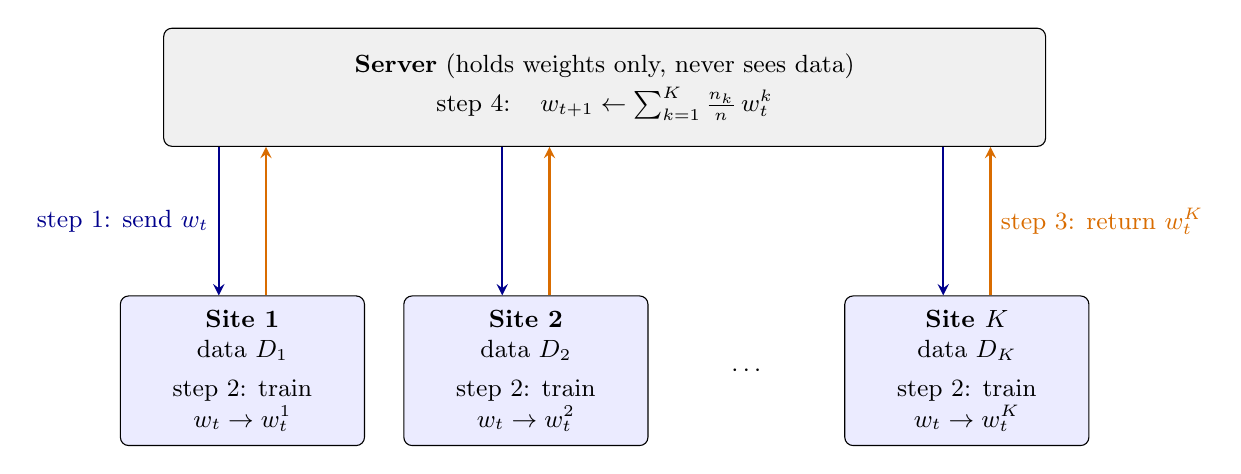
\begin{tikzpicture}[
    font=\small,
    box/.style={draw, rounded corners=3pt, align=center},
    servernode/.style={box, fill=gray!12, minimum width=11.2cm, minimum height=1.5cm},
    clientnode/.style={box, fill=blue!8, minimum width=3.1cm, minimum height=1.9cm},
    down/.style={-stealth, thick, draw=blue!55!black},
    up/.style={-stealth, thick, draw=orange!85!black}
]
\node[servernode] (srv) at (0, 3.6)
  {\textbf{Server} (holds weights only, never sees data)\\[2pt]
   step 4: \; $w_{t+1} \gets \sum_{k=1}^{K} \frac{n_k}{n} \, w_t^{k}$};
\node[clientnode] (c1) at (-4.6, 0)
  {\textbf{Site 1}\\ data $D_1$\\[3pt] step 2: train\\ $w_t \to w_t^{1}$};
\node[clientnode] (c2) at (-1.0, 0)
  {\textbf{Site 2}\\ data $D_2$\\[3pt] step 2: train\\ $w_t \to w_t^{2}$};
\node at (1.8, 0) {$\cdots$};
\node[clientnode] (cK) at (4.6, 0)
  {\textbf{Site $K$}\\ data $D_K$\\[3pt] step 2: train\\ $w_t \to w_t^{K}$};
\draw[down] ([xshift=-3mm]srv.south -| c1) -- ([xshift=-3mm]c1.north)
    node[midway, left, text=blue!55!black] {step 1: send $w_t$};
\draw[up] ([xshift=3mm]c1.north) -- ([xshift=3mm]srv.south -| c1);
\draw[down] ([xshift=-3mm]srv.south -| c2) -- ([xshift=-3mm]c2.north);
\draw[up] ([xshift=3mm]c2.north) -- ([xshift=3mm]srv.south -| c2);
\draw[down] ([xshift=-3mm]srv.south -| cK) -- ([xshift=-3mm]cK.north);
\draw[up] ([xshift=3mm]cK.north) -- ([xshift=3mm]srv.south -| cK)
    node[midway, right, text=orange!85!black] {step 3: return $w_t^{K}$};
\end{tikzpicture}
\caption{One round of federated averaging (FedAvg). The server sends the current global weights $w_t$ to every site (step 1). Each site trains the model on its own data for $E$ epochs (step 2) and sends the resulting local weights back (step 3). The server averages the local models, weighting each site by its share of the data, to produce the next global model $w_{t+1}$ (step 4). Raw data never moves. Rounds repeat until the model stops improving.}
\label{fig:fedavg-round}
\end{figure}

\subsection{Why local epochs matter}

The number of local epochs $E$ controls a trade-off. Consider the simplest case first. Suppose each site took a single gradient step on its full local dataset, so $w_t^{k} = w_t - \eta \nabla F_k(w_t)$. The server's average would then be
\begin{equation}
\label{eq:fl-fedsgd}
\sum_{k=1}^{K} \frac{n_k}{n} \, w_t^{k}
\;=\; w_t - \eta \sum_{k=1}^{K} \frac{n_k}{n} \nabla F_k(w_t)
\;=\; w_t - \eta \, \nabla f(w_t).
\end{equation}
This is exactly one gradient descent step on the pooled objective $f(w)$. The variant that works this way is called FedSGD. It behaves like centralised training, but it needs one round of communication for every single gradient step, which is far too slow in practice. FedAvg instead lets each site take many steps per round. This cuts the number of rounds needed by one to two orders of magnitude \citep{mcmahan2017fedavg}.

The saving has a price when sites differ. During its $E$ epochs, each local model fits its own site's data and the local models move apart. Their average is then no longer a gradient step on $f(w)$, and Eq.~\ref{eq:fl-fedsgd} no longer holds. Training can converge slowly or settle on a worse model \citep{li2020fedprox}. This effect is called client drift. It is the training-time face of the domain shift problem described in Section~\ref{sec:intro-shift}, and most of the FedAvg variants in this report exist to manage it. Section~\ref{sec:rel-dg} presents them.

\subsection{Cross-device and cross-silo federation}

In the original FedAvg paper the clients were mobile phones. There were very many, they dropped in and out, and only a small random fraction took part in each round. That setting is called cross-device. A federation of hospitals is the other setting, called cross-silo \citep{kairouz2021advances}. The sites are few, known, and reliable, and all of them take part in every round. All the federated work in this report is cross-silo, so client sampling plays no role and Eq.~\ref{eq:fl-agg} always sums over all $K$ sites.

One caution belongs here. Keeping raw data local removes the need to share records, but sharing model weights is not the same as sharing nothing. What weight sharing can still leak, and what can be done about it, is covered in Section~\ref{sec:rel-privacy}.

\section{Domain shift and generalisation}
\label{sec:rel-dg}
\outline{Why a model degrades on new sites. Held-in versus out-of-distribution testing. Personalisation versus one shared model. This is where the FedAvg variants now go: FedProx, MLDG, APFL, Ditto, each in one or two plain sentences before any maths, placed next to the problem it solves.}

\section{AI for ophthalmic imaging}
\label{sec:rel-eye}
\outline{Modalities (fundus, OCT), screening tasks, foundation models such as RETFound.}

\section{Blood glucose forecasting}
\label{sec:rel-glucose}
\outline{CGM data, the 30 and 60 minute tasks, from classical models to transformers.}

\section{Privacy}
\label{sec:rel-privacy}
\outline{What FL does and does not protect against. Differential privacy, secure aggregation, attacks.}
